%--------------------------------------------------------------
% thesis.tex 
%--------------------------------------------------------------
% - template for the main file of Informatica@Unifi Thesis 
% - based on Classic Thesis Style Copyright (C) 2008 
%   Andr\'e Miede http://www.miede.de   
%--------------------------------------------------------------
\documentclass[openright,titlepage,oneside,fleqn,
	headinclude,12pt,a4paper,footinclude,makeidx]{scrbook}%twoside
%--------------------------------------------------------------
\usepackage[italian]{babel}
\usepackage[utf8]{inputenc} 
\usepackage[T1]{fontenc} 
\usepackage[square,numbers]{natbib} 
\usepackage[fleqn]{amsmath}  
\usepackage{ellipsis}
\usepackage{listings}
\usepackage{subfig}
\usepackage[format=plain,labelformat=simple,labelsep=colon]{caption}
\usepackage{appendix}
\usepackage{siunitx}
\usepackage{lipsum}
\usepackage{dia-classicthesis-ldpkg}
\usepackage[eulerchapternumbers,linedheaders,subfig,beramono,eulermath,
parts,dottedtoc]{classicthesis}
\usepackage{imakeidx}
\usepackage{wrapfig}
\usepackage[italian,noabbrev]{cleveref}
%---------------------------------------------------------------
\newcommand{\myItalianTitle}{Titolo italiano\xspace}
\newcommand{\myEnglishTitle}{Titolo inglese\xspace}
\newcommand{\myDegree}{Corso di Laurea Magistrale in Informatica\xspace}
\newcommand{\myCurriculum}{Resilient and secure cyberphysical systems\xspace}
\newcommand{\myName}{Marco Buracchi\xspace}
\newcommand{\myProf}{Michele Boreale\xspace}
\newcommand{\myFaculty}{Scuola di Scienze Matematiche, Fisiche e Naturali\xspace}
\newcommand{\myUni}{\protect{Università degli Studi di Firenze}\xspace}
\newcommand{\myLocation}{Firenze\xspace}
\newcommand{\myTime}{Anno Accademico 2017-2018\xspace}
\newcommand{\mycopyright}{
\includegraphics[width=1.5cm]{logo/cc.png} 
	\href{https://creativecommons.org/licenses/by-nc-sa/4.0/}{Creative
		Commons Attribution-NonCommercial-ShareAlike 4.0 International (CC BY-NC-SA 4.0)  }\xspace}
\newcommand{\disps}{dispositivo crittografico }
\newcommand{\dispp}{dispositivi crittografici }
\newcommand{\codice}[4]{\lstinputlisting[language={C},firstline={#1}, lastline={#2},caption={#3},label={#4}]{"D:/UNIFI/Magistrale/Tesi/spectre/primeProbe/spark.c"}}
\newcommand{\myfloatalign}{\centering} 

\renewcommand{\lstlistingname}{Codice}% Listing -> Codice
%--------------------------------------------------------------
\newlength{\abcd} % for ab..z string length calculation
% how all the floats will be aligned
\setlength{\extrarowheight}{3pt} % increase table row height
\captionsetup{format=hang,font=small}
%--------------------------------------------------------------
% Layout setting
%--------------------------------------------------------------
\graphicspath{{img/}}
\usepackage{geometry}
\geometry{
	a4paper,
	ignoremp,
	bindingoffset = 1cm, 
	textwidth     = 13.5cm,
	textheight    = 21.5cm,
	lmargin       = 3.5cm, % left margin
	tmargin       = 4cm    % top margin 
}

\crefname{listing}{codice}{codici}

\lstset{ %
	%backgroundcolor=\color{back},	% choose the background color; you must add \usepackage{color} or \usepackage{xcolor}; should come as last argument
	basicstyle=\footnotesize,  		% the size of the fonts that are used for the code
	breakatwhitespace=false,        % sets if automatic breaks should only happen at whitespace
	breaklines=true,                % sets automatic line breaking
	captionpos=b,                   % sets the caption-position to bottom
	commentstyle=\color{gray},   	% comment style
	frame=rlbt,	         	        % adds a frame around the code
	frameround=fttt					% round corner (use f instead t to edge corner)
	keepspaces=true,                % keeps spaces in text, useful for keeping indentation of code (possibly needs columns=flexible)
	keywordstyle=\color{blue},      % keyword style
	language=C,               % the language of the code
	numbers=left,                   % where to put the line-numbers; possible values are (none, left, right)
	numbersep=5pt,                  % how far the line-numbers are from the code
	numberstyle=\scriptsize\color{black}, % the style that is used for the line-numbers
	rulecolor=\color{black},        % if not set, the frame-color may be changed on line-breaks within not-black text (e.g. comments (green here))
	showspaces=false,               % show spaces everywhere adding particular underscores; it overrides 'showstringspaces'
	showstringspaces=false,         % underline spaces within strings only
	showtabs=false,                 % show tabs within strings adding particular underscores
	stepnumber=1,                   % the step between two line-numbers. If it's 1, each line will be numbered
	stringstyle=\color{OrangeRed},  % string literal style
	tabsize=2                   	% sets default tabsize to 2 spaces
}

\makeindex[intoc]
%--------------------------------------------------------------
\begin{document}
\frenchspacing
\raggedbottom
\pagenumbering{roman}
\pagestyle{plain}
%--------------------------------------------------------------
% Frontmatter
%--------------------------------------------------------------
%--------------------------------------------------------------
% titlepage.tex (use thesis.tex as main file)
%--------------------------------------------------------------
\begin{titlepage}
	\begin{center}
   	\large
      \hfill
      \vfill
      \begingroup
         
\includegraphics[scale=0.15]{logo/LOGO}\\
%			\spacedallcaps{\myUni} \\ 
			\myFaculty \\
			\vspace{0.5cm}
			\myDegree \\ 
			Curriculum: \emph{\myCurriculum}\\
			\vspace{0.5cm}
         \vspace{0.5cm}    
         Tesi di Laurea Magistrale 
      \endgroup 
      \vfill 
      \begingroup
      	\color{Maroon}\spacedallcaps{\myItalianTitle} \\ $\ $\\
      	\spacedallcaps{\myEnglishTitle} \\ 	
	\bigskip
      \endgroup
      \spacedlowsmallcaps{\myName}
      \vfill 
      \vfill
      Relatore: Prof. \emph{\myProf}\\
      \vfill
      \vfill
      \myTime
      \vfill                      
	\end{center}        
\end{titlepage}   
%--------------------------------------------------------------
% back titlepage
%--------------------------------------------------------------
   \newpage
	\thispagestyle{empty}
	\hfill
	\vfill
	\noindent\myName: 
	\textit{\myItalianTitle,} 
	\myDegree, \mycopyright, \myUni, \myTime
%--------------------------------------------------------------
% back titlepage end
%--------------------------------------------------------------
\pagestyle{scrheadings}
%--------------------------------------------------------------
% Mainmatter
%--------------------------------------------------------------
\pagenumbering{arabic}
\tableofcontents
\listoffigures
\lstlistoflistings
\listoftables
\cleardoublepage
\thispagestyle{empty}
\begin{flushright}
\null\vspace{\stretch {1}}
\emph{"Da campo a campo, nel tetro grembo della notte,\\s’avverte appena il brusio di entrambe le armate,\\sicché le sentinelle appostate quasi possono udire\\i mormorii furtivi delle sentinelle nemiche" \break --- Enrico V, William Shakespear} \vspace{\stretch{2}}\null
\end{flushright}
\cleardoublepage
%----------------CAPITOLI--------------------------------------
\chapter{Introduzione}
	prova \cite{kocher2018spectre}.

\chapter{Side-channel attacks}

	I \emph{side-channel attacks} sono metodi di criptanalisi che sfruttano le side-channels informations insieme ad altre tecniche di analisi per recuperare la chiave utilizzata da un \disps\cite{standaert2010introduction}.\begin{figure}
		
		\begin{center}
			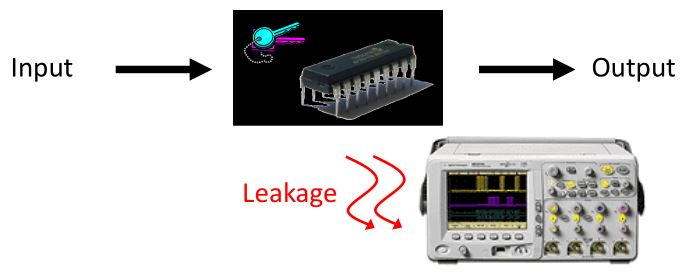
\includegraphics[scale=.6]{sideChannelLeakage}
			\caption{Esempio di side-channel attack}
			\label{fig:attack}
		\end{center}
	\end{figure}
	
	Nella \cref{fig:attack} si può vedere una configurazione tipo di side-channel attack. Da una parte c'è il dispositivo che implementa la funzione crittografica e accanto c'è lo strumento utilizzato per rilevare le grandezze fisiche prodotte dal dispositivo attaccato. La cosa fondamentale è che questo tipo di attacchi non vanno a colpire direttamente la funzione crittografica ma sfruttano le informazioni fisiche dell'ambiente intorno al dispositivo.
	
	L'analisi di questi metodi ha acquisito notevole interesse dato che questo tipo di attacchi possono essere montati velocemente e molto spesso non richiedono hardware particolare e costoso. Con pochi euro si possono ad esempio acquistare in comuni negozi di bricolage o elettronica apparecchi in grado di analizzare il consumo elettrico di un dispositivo. Con tali apparecchi è possibile montare in pochi secondi un attacco di tipo \emph{Simple Power Analysis}\cite{mangard2002simple} che verrà spiegato più avanti. 
	
	Il governo degli USA, nel suo "Orange book"\cite{latham1986department} indica dei requisiti di sicurezza per i sistemi operativi. Questo documento introduce i primi standard per l'\emph{information leakage}. Purtroppo la letteratura specializzata è però molto variegata e disomogenea quindi, come prima cosa, cerchiamo di trovare un modo per classificare i vari tipi di attacchi in maniera tale da avere una visione più sistemistica del settore.
	
	\section{Background}
	
		In questa sezione verranno stabiliti dei parametri per classificare i vari tipi di attacchi side-channel.
	
		\subsection{Tipi di canali}
	
			Nel lavoro di \emph{Ge, Yarom, Cock e Heiser}\cite{ge2016survey} vengono fornite alcune definizioni che utilizzeremo nel prosieguo di questa tesi. La prima distinzione che è necessario fare è quella tra side-channel e \emph{covert-channel}. Con i primi ci si riferisce ai canali che lasciano \emph{accidentalmente} filtrare informazioni sensibili (ad esempio una chiave crittografica) in una comunicazione tra due partecipanti fidati. I secondi sono quelli creati e sfruttati dall'attaccante ad esempio tramite l'utilizzo di Trojan e che \emph{deliberatamente} lasciano filtrare le informazioni. In questo lavoro verranno trattati solamente i primi.
			
			L'altra differenza fondamentale per quello che riguarda i canali è quella tra canali di tipo \emph{storage} e canali di tipo \emph{timing}. I canali di tipo storage vengono sfruttati per ottenere qualcosa di direttamente visibile nel sistema (valore dei registri, valore di ritorno di una system call, ecc.). Quelli di tipo timing vengono sfruttati andando ad osservare variazioni del tempo di esecuzione di un programma (o di parti di esso).
			
		\subsection{Tipi di attacco}
		
			\emph{Standaert} nel suo lavoro \cite{standaert2010introduction} utilizza altre due dimensioni interessanti per classificare questi attacchi; l'\emph{invasività} e l'\emph{attività}. 
			
			Si definisce invasivo un attacco che richiede un disassemblamento del dispositivo attaccato per avere accesso diretto ai suoi componenti interni (wiretapping o sensori collegati direttamente all'hardware). Un attacco non invasivo, al contrario, sfrutta solamente le informazioni disponibili esternamente (quasi sempre involontarie) come il tempo d'esecuzione o l'energia consumata.
			
			Si definisce attivo un attacco che cerca di interferire con il corretto funzionamento del dispositivo (fault-injection) mentre un attacco passivo si limita ad osservare il comportamento del dispositivo durante il suo lavoro senza disturbarlo. 
			
		\subsection{Grandezza fisica osservata}
		
			Una caratteristica principale di questi attacchi è sicuramente la grandezza fisica che viene osservata per montare l'attacco. Teoricamente, qualunque grandezza fisica misurabile può essere sfruttata ma alcune si prestano maggiormente rispetto ad altre. 
			
			Il tempo e il consumo energetico sono le più sfruttate ma non sono di certo le uniche. \emph{Genkin, Shamir e Tromer} nel loro lavoro \cite{genkin2014rsa} vanno ad ascoltare i rumori prodotti dal processore. \emph{Ferrigno e Hlavac}\cite{ferrigno2008aes} osservano la luce (qualche fotone) emessa dai transistor nel passaggio di stato da 0 a 1. \emph{Martinasek, Zeman e Trasy} sfruttano i campi elettromagnetici creati dai chip. \emph{Giraud}\cite{giraud2004dfa} sfrutta la tecnica della fault-injection e analizza i risultati delle computazioni.
			
			Questo elenco assolutamente non esaustivo delle tecniche utilizzate può far capire quanto variegato ed eterogeneo (nonché in continua evoluzione) sia questo settore.
			
			Tutti questi attacchi (e anche altri) verranno approfonditi più avanti.
			
		\subsection{Hardware attaccato}
		
			Gli attacchi possono essere suddivisi anche in base alla componente hardware che viene attaccata. Anche in questo caso ci sono componenti più attaccati di altri (cache e processori) ma non mancano esempi di attacchi a monitor\cite{van1985electromagnetic}, tastiere\cite{asonov2004keyboard} o stampanti\cite{backes2010acoustic}.
			
		\subsection{Algoritmo attaccato}
		
			Un'ultima classificazione può essere effettuata andando a discriminare gli attacchi secondo l'algoritmo crittografico attaccato. In questo caso i due maggiori algoritmi attaccati sono senza dubbio AES ed RSA.
			
			\begin{table}[]
				\centering
				\caption{Classificazione dei principali attacchi analizzati}
				\label{tab:attacchi}
				\begin{tabular}{c|c|c|c|c|c} \hline
					Articolo 					& Grandezza                    & Hardware   & Algoritmo & Invasivo & Attivo \\ \hline
					\cite{genkin2014rsa}		& Suono                        & CPU        & RSA       & No       & No     \\ \hline
					\cite{ferrigno2008aes}		& Luce                         & Transistor & AES       & Sì       & No     \\ \hline
					\cite{kocher2018spectre}	& Tempo                        & Cache      & RSA       & No       & No     \\ \hline
					\cite{mangard2002simple}	& Consumo elettrico            & Smartcard  & AES       & No       & No     \\ \hline
					\cite{martinasek2012simple}	& Campo elettromagnetico       & Chip       & AES       & No       & No     \\ \hline
					\cite{giraud2004dfa}		& Risultato della computazione & Smartcard  & AES       & Sì       & Sì    
				\end{tabular}
			\end{table}
		
			Nella \cref{tab:attacchi} si è provato a classificare con i criteri sopra definiti i 6 attacchi che verranno approfonditi in questo lavoro.
			
	\section{Attacchi basati sul suono}
	\lipsum[1-5]
	\section{Attacchi basati sulla luce}
	\lipsum[1-5]
	\section{Attacchi basati sul tempo}
	\lipsum[1-5]
	\section{Attacchi basati sul consumo elettrico}
	\lipsum[1-5]
	\section{Attacchi basati sul campo elettromagnetico}
	\lipsum[1-5]
	\section{Attacchi basati sui risultati delle computazioni}
	\lipsum[1-5]
\chapter{Timing attacks}
	\index{Timing attacks}Come anticipato nel capitolo precedente, approfondiremo adesso la tipologia di attacchi basati sul tempo focalizzandoci maggiormente su quelli che hanno come obiettivo la cache del processore. 
	
	L'idea di base che sta sotto i timing attacks è quella che l'esecuzione di un determinato programma, al variare delle operazioni che vengono eseguite e al variare degli input, impiega tempi diversi per portare a termine il proprio compito.
	
	\lstinputlisting[language={Java},caption={Esempio di funzione vulnerabile ad un timing attack},label={list:timingBase}]{code/timingBase.txt}
		
	Ad esempio il \cref{list:timingBase} se fatto girare con la stringa ("passwordToBeStolen") impiegherà un tempo maggiore rispetto allo stesso programma fatto girare con la stringa ("foo"). Nel primo caso infatti verrà scansionata tutta la stringa mentre nel secondo caso si interromperà immediatamente. Questa informazione può essere utilizzata dall'attaccante per capire la stringa esatta. Per portare questo concetto al livello che ci interessa vediamo prima delle nozioni fondamentali sulla cache del processore. 
	
	\section{La cache del processore}
		Dato che la differenza di velocità tra le memorie e la capacità di calcolo dei processori aumenta sempre di più \cite{hennessy2011computer} la banda del bus di comunicazione e la velocità di accesso alla memoria principale sono diventati un fattore limitante sul throughput generale del processore. Questo collo di bottiglia viene attenuato dall'utilizzo delle cache\index{Cache}. 
		
		La cache è infatti un piccolo banco di memoria molto veloce sito all'interno di ogni core che il processore utilizza per immagazzinare i valori delle celle di memoria accedute più recentemente. 
		
		\subsection{Struttura della cache}
			I processori moderni hanno generalmente due livelli di cache per ogni core chiamati rispettivamente L1 e L2 ed un terzo livello chiamato \ac{LLC} o L3 condiviso tra i tutti i core (nella \cref{tab:processori} sono riportate le dimensioni delle varie memorie di alcuni processori). 
			
			\begin{table}[]
				\footnotesize
				\centering
				\begin{tabular}{|c|c|c|c|c|c|c|} \hline
					Casa		& Nome			& Core	& L1			& L2			& L3		& Prezzo (\$)	\\ \hline \hline
					Intel		& i3-530		& 2		& 2 x 64 KB		& 2 x 512KB		& 1 x 4 MB	& 113			\\ \hline
								& i5-6685R		& 4		& 4 x 64 KB		& 4 x 256KB		& 1 x 6 MB	& 288			\\ \hline
								& i7-6950X		& 10	& 10 x 64 KB	& 10 x 256KB	& 1 x 25 MB	& 1723			\\ \hline
								& i9-8950HK		& 6		& 6 x 64 KB		& 6 x 256KB		& 1 x 12 MB	& 583			\\ \hline
					AMD			& A4 Pro-3350B	& 4		& 4 x 64 KB		& 1 x 2MB		& -			& -				\\ \hline
								& Athlon 5370	& 4		& 4 x 64 KB		& 1 x 2MB		& -			& 55			\\ \hline
								& Epyc 7251		& 8		& 8 x 96 KB		& 8 x 512KB		& 32 MB		& 475			\\ \hline
				\end{tabular}
				\caption{Caratteristiche di alcuni processori}
				\label{tab:processori}
			\end{table}
			
			Considerando che l'accesso alla memoria principale in media impiega dai 50 ai 150 \emph{ns} mentre l'accesso alla cache L1 utilizza un tempo nell'ordine degli 0.3 \emph{ns} si può capire l'enorme differenza di prestazioni che possono essere raggiunte utilizzando questo tipo di memoria.
		
			Nella \cref{fig:cachei5} si può vedere l'architettura del processore quadcore Intel Core i5-3470. La gerarchia delle cache è organizzata in una memoria L1 di 64KB (divisa in 32KB per le istruzioni e 32KB per i dati), una memoria L2 da 256KB ed una memoria L3 da 6MB.
			
			\begin{figure}
				\begin{center}
					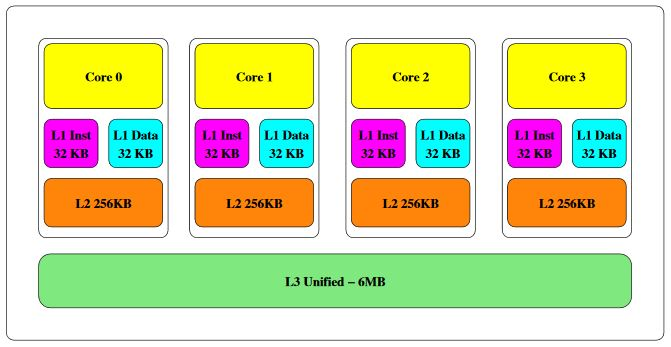
\includegraphics[scale=0.6]{cachei5}
					\caption{Architettura del processore Intel Core i5-3470}
					\label{fig:cachei5}
				\end{center}
			\end{figure}
			
			Andiamo ad analizzare più nel dettaglio le caratteristiche di una singola cache\cite{ge2016survey,yarom2014flush+}.
			
			\subsubsection{Cache lines}
				\index{Cache lines}Per sfruttare la località spaziale le caches sono divise in lines. Una cache line contiene un blocco di bytes adiacenti (generalmente di dimensione congrua ad una potenza di 2) caricati dalla memoria. Se uno qualunque dei bytes deve essere rimosso (si parla di \emph{evicting}) per far spazio ad un altro dato, tutta la line viene ricaricata.
				
			\subsubsection{Associatività}
				Teoricamente una qualunque posizione di memoria può essere mappata in una qualunque cache line ed una cache ad \emph{n} lines potrebbe contenere \emph{n} linee qualunque dalla memoria. Questo tipo di cache viene chiamato \emph{fully-associative cache}\index{Fully-associative cache} ed è la migliore in teoria perché può sempre essere usata al massimo delle sue capacità e i cache miss si hanno solamente quando non c'è più spazio libero nella cache. In pratica però questo si traduce in un controllo in parallelo di tutte le linee che aumenta la complessità architetturale e il consumo di energia.
				
				L'estremo opposto è chiamato \emph{direct-mapped cache}\index{Direct-mapped cache}. In questo sistema ogni locazione di memoria può stare in una sola cache line, ben determinata da una funzione di indicizzazione. Due locazioni di memoria che mappano sulla stessa cache line non possono essere immagazzinate contemporaneamente e il loading di una comporta inevitabilmente l'evicting dell'altra. Questo potrebbe portare ad avere dei miss anche con la cache semivuota.
				
				Concretamente viene utilizzata una via di mezzo tra queste due soluzioni chiamata \emph{set-associative cache}\index{Set-associative cache}. La cache viene divisa in \emph{sets} (generalmente di dimensione compresa tra 2 e 24 lines) in cui ogni indirizzo viene controllato in parallelo come in una fully-associative cache. In quale set viene mappato un blocco di memoria viene calcolato come per una direct-mapped cache da una funzione del suo indirizzo. Una cache con \emph{n} line sets viene chiamata \emph{n-way associative} (\cref{fig:cachefill}).
				
				Si può notare che le direct-mapped e le fully-associative cache non sono altro che casi particolari di set-associative cache rispettivamente 1-way associative ed N-way associative (dove N è il numero di linee della cache).
				
				\begin{figure}
					\begin{center}
						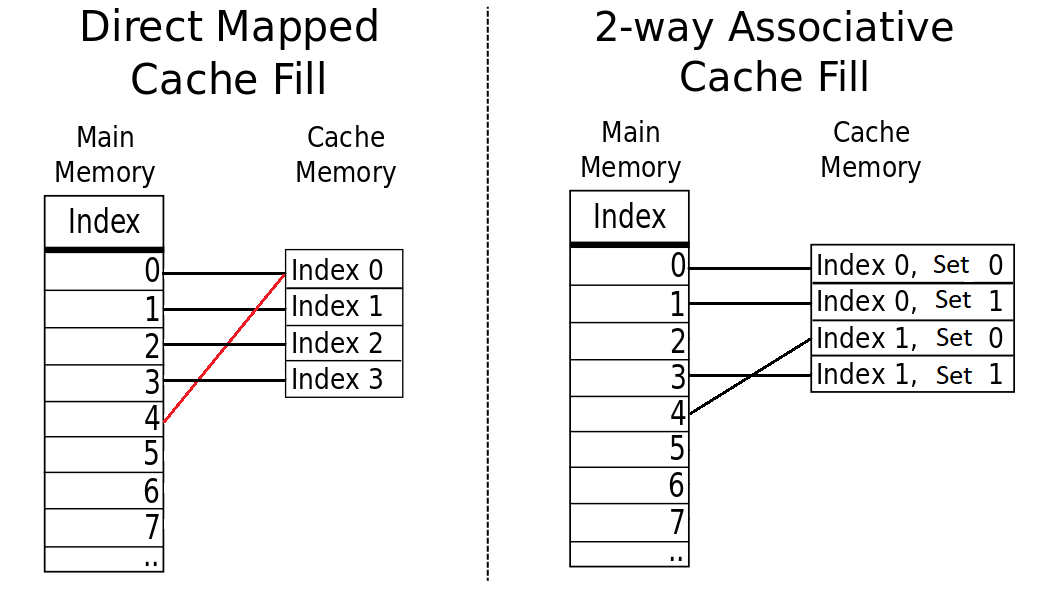
\includegraphics[scale=.35]{cachefill}
						\caption{Schemi di associatività della cache.}
						\label{fig:cachefill}
					\end{center}
				\end{figure}
				
			\subsubsection{Inclusività}
				Una caratteristica che verrà sfruttata per montare l'attacco è l'\emph{inclusività}\index{Inclusività}. 
				
				Ogni livello superiore di cache contiene un sottoinsieme dei dati contenuti dal livello direttamente inferiore. Per mantenere questa caratteristica, quando viene eseguito un evicting di un dato da un livello inferiore, questo viene rimosso anche da tutti i livelli superiori.
				
	\section{Cache attacks}
		Per capire come funzionano la maggior parte degli attacchi alle cache prendiamo in considerazione un array di dati. Quando un elemento di questo array viene acceduto possono verificarsi una di queste due condizioni:
		
		\begin{enumerate}
			\item Il dato è presente in cache, si verifica una hit e viene recuperato molto velocemente.
			\item Il dato non è presente in cache, si verifica una miss e bisogna aspettare che venga recuperato dalla memoria principale.
		\end{enumerate}
		
		La differenza tra le due esecuzioni è notevole (diversi ordini di grandezza) ed è questa l'informazione utilizzata nell'attacco.
		
		\subsection{Tassonomia}
			Una prima classificazione dei cache attacks si basa sullo stato della cache al momento dell'attacco\cite{canteaut2006understanding}.
			
			\begin{itemize}
				\item \emph{Empty initial state}\index{Empty initial state} (reset attacks): questi attacchi si basano sull'assunzione che nessun dato che dovrà essere utilizzato dalla vittima è presente in cache.
				\item \emph{Forged initial state}\index{Forged initial state} (initialization attacks): in questo caso l'attaccante deve essere in grado di portare la cache in uno stato noto prima di poter effettuare l'attacco.
				\item \emph{Loaded initial state}\index{Loaded initial state} (micro-architecture attacks): la cache contiene tutti i dati necessari alla vittima per eseguire il programma.
			\end{itemize}
		
			Nello stesso lavoro si fornisce una classificazione anche in base al tipo di cache miss. 
			
			\begin{itemize}
				\item \emph{Cold start misses}\index{Cold start misses}: questo tipo di miss si ottiene quando il dato viene acceduto per la prima volta e quindi non è ancora mai stato caricato in cache.
				\item \emph{Capacity misses}\index{Capacity misses}: questo tipo di miss si ottiene quando si cerca di accedere a porzioni di memoria più grandi della dimensione della cache che quindi non possono essere presenti contemporaneamente.
				\item \emph{Conflict misses}\index{Conflict misses}: questo tipo di miss si ottiene quando un accesso precedente alla nostra richiesta ha provocato la eviction del dato di interesse (che era presente in cache).
			\end{itemize}
			
			In \cite{lipp2016armageddon,ge2016survey} si classificano gli attacchi in base all'approccio utilizzato:
			
			\begin{figure}
				\begin{center}
					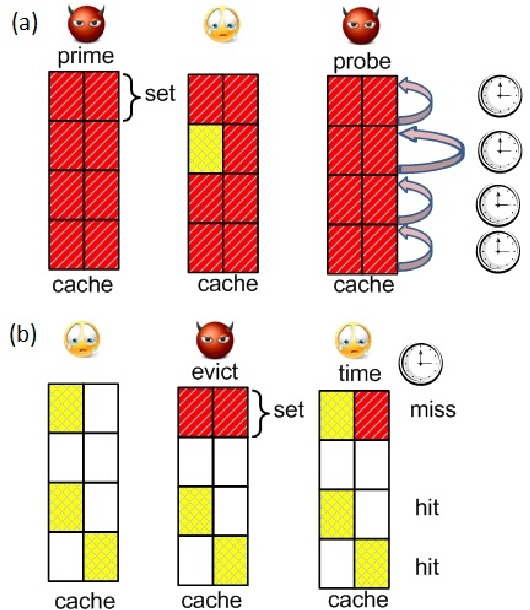
\includegraphics[scale=0.4]{cacheattacks}
					\caption{Schema di attacco Prime+Probe (a) e Evict+Time(b)}
					\label{fig:cacheattacks}
				\end{center}
			\end{figure}
			
			\begin{itemize}
				\item \emph{Prime+Probe}\cite{osvik2006cache}\index{Prime+Probe}: Questo è un attacco di tipo forged initial state. L'attaccante precarica uno o più set della cache con dati propri. Dopo l'esecuzione della funzione vittima prova a riaccedere ad i propri dati. Se la funzione vittima non ha utilizzato lines mappate nei cache set occupati dall'attaccante, egli otterrà solo cache hit. Al contrario, se c'è stato l'evict di qualche line allora capirà quale ha utilizzato la vittima. Lo schema di questo attacco e del seguente è visibile in \cref{fig:cacheattacks}.
				\item \emph{Evict+Time}\cite{osvik2006cache}\index{Evict+Time}: Questo attacco è di tipo loaded initial state e suppone che tutti i dati che servono alla vittima siano già in cache. Questa condizione può essere ottenuta facendo eseguire una prima volta la funzione vittima. Con questa base, l'attaccante fa eseguire la funzione alla vittima calcolandone il tempo di esecuzione. Successivamente esegue una evict di un cache set caricando dati propri e fa eseguire nuovamente la funzione vittima. Se il tempo di questa ultima esecuzione è maggiore del precedente vuol dire che la funzione ha cercato di utilizzare il dato che è stato rimosso dalla cache ed ha dovuto aspettare di recuperarlo dalla memoria principale.
				\item \emph{Flush+Reload}\cite{yarom2014flush+}\index{Flush+Reload}: Questo attacco è una variante di Prime+Probe. L'attacco si divide in tre fasi. Nella prima fase l'attaccante esegue l'evict della linea a cui è interessato utilizzando l'istruzione \emph{clflush} che invalida il dato su tutti i livelli della cache. Nella seconda fase aspetta che la vittima esegua la propria funzione. Nella terza fase l'attaccante ricarica la linea che aveva rimosso. Se la risposta è veloce vuol dire che la vittima l'ha portata in cache durante l'esecuzione della sua funzione.
				\item \emph{Evict+Reload}\cite{gruss2015cache}\index{Evict+Reload}: Una variante del Flush+Reload che utilizza la eviction al posto dell'istruzione di flush. Questa variante è poco utile se il processore sotto attacco è della famiglia x86 in quanto l'istruzione \emph{clflush} non richiede alcun privilegio mentre assume un certo rilievo se l'obiettivo è quello di attaccare un processore che non fornisce, nel suo set di istruzioni, una istruzione non privilegiata in grado di rimuovere dati dalla cache (come ad esempio quelli della famiglia ARM).
				\item \emph{Flush+Flush}\cite{gruss2016flush+}\index{Flush+Flush}: Diversamente da tutti i precedenti approcci, in questo caso non si esegue nessun accesso alla memoria ma l'attaccante si basa solamente sul tempo impiegato dall'istruzione \emph{clflush}. In \cite{lipp2016armageddon} si fa vedere come l'esecuzione di questa funzione abbia tempi differenti se chiamata su un indirizzo presente in cache o meno.  
			\end{itemize}
		
		\section{Contromisure possibili}
			Le difese da questo tipo di attacchi sono sia software che hardware e si dividono in 5 grandi famiglie\cite{ge2016survey}
			
			\begin{description}
				\item[Tecniche a tempo costante:] L'idea di base è quella di rendere il comportamento del codice che esegue operazioni critiche indipendente dai dati. Per esempio cercare di rendere una funzione crittografica indipendente sia dalla chiave che dall'input. Questo può essere ottenuto facendo eseguire istruzioni inutili per uniformare il tempo di esecuzione o accedendo a dati casuali dalla memoria per confondere l'attaccante sull'utilizzo della cache. 
				
				Queste soluzioni ovviamente portano ad una drastica perdita di prestazioni. Il tempo di esecuzione dovrà infatti tendere al tempo di esecuzione massimo ogni volta che sarà necessario richiamare la funzione.
				
				L'altro grande problema di questo tipo di soluzioni è quello della differenza di risultati su hardware differenti. Ad esempio \emph{Cock et al.}\cite{cock2014last} hanno dimostrato che la correzione a tempo costante adottata per mitigare l'attacco \emph{Lucky 13}\cite{al2013lucky} in OpenSSL 1.0.1e non risolve il problema se fatto girare su un processore ARM AM3358. 
				\item[Inserimento di rumore:] Questa famiglia di contromisure tende a rendere inutilizzabili le misure ottenute dall'attaccante inserendo in ogni evento osservabile da qualsiasi processo una quantità di rumore tale da renderne impossibile una qualunque analisi\cite{hu1992reducing}. Questa soluzione, in teoria, riesce a risolvere completamente il problema ma è stato dimostrato\cite{cock2014last} che in pratica non è applicabile. La quantità di rumore da produrre e da aggiungere alla computazione è talmente elevata che il sistema impiegherebbe la maggior parte delle sue risorse in questa operazione piuttosto che nella effettiva computazione del programma.
				\item[Imporre determinismo:] In questo caso si cerca di eliminare qualsiasi tipo di misura sul tempo eliminando completamente le variazioni di tempo visibile. Ad esempio in \cite{aviram2012efficient} si propone di eliminare completamente l'accesso al tempo reale fornendo all'esterno solamente un clock virtuale il cui avanzamento è completamente deterministico e indipendente dalle azioni di componenti vulnerabili. Per ottenere questo risultato si cerca di sincronizzare tutti i clock con l'esecuzione di un singolo processo, indipendente da input o azioni esterne, che esegue in tempo costante.
				\item[Suddividere il tempo:] In questo caso si cerca di suddividere il tempo in sezioni nelle quali si fornisce un accesso esclusivo all'hardware condiviso. Ci sono diverse tecniche per ottenere questo risultato uno dei quali è la cancellazione completa della cache ad ogni context switch(\emph{cache flushing}\index{Cache flushing}\cite{zhang2013duppel}). Questo ovviamente porta ad una perdita in prestazioni molto grande e si è passati al \emph{lattice scheduling}\index{Lattice scheduling}\cite{denning1976lattice} che esegue il flushing della cache non ad ogni context switch ma solo nel passaggio da processi sensibili a processi inaffidabili. Un'altra soluzione\cite{varadarajan2014scheduler} mira a sfruttare la necessità di analizzare molto spesso lo stato della cache della vittima che hanno attacchi di tipo Prime+Probe ad esempio. Questa necessità non viene alimentata imponendo un tempo minimo di esecuzione per le componenti vulnerabili entro il quale non possono essere prelazionate.
				\item[Suddividere le risorse hardware:] Attacchi eseguiti da processi concorrenti possono essere evitati solamente suddividendo adeguatamente le risorse hardware tra i vari processi. Per quanto riguarda la cache sono state avanzate varie proposte. Percival\cite{percival2005cache} suggerisce di suddividere la cache L1 tra i vari processi in modo tale da non permettere ad un processo di accedere o rimuovere lines utilizzate da un altro. Wang and Lee\cite{wang2007new} propongono invece la \emph{partition-locked cache}, un meccanismo hardware che permette di assegnare dei lock ad alcune lines contenenti dati particolarmente sensibili in maniera tale da non poter essere rimosse (ad esempio le tabelle di lookup di \ac{AES}).				 
			\end{description}
\chapter{SPECTRE attacks}

	\begin{wrapfigure}{l}{0.4\textwidth}
		
\includegraphics[width=0.38\textwidth]{spectre}
		\caption{Il logo di SPECTRE}
		\label{fig:spectre}
	\end{wrapfigure}

	\index{Spectre}In questo capitolo verrà presentato il progetto \emph{SPECTRE}\cite{kocher2018spectre} (il cui logo è rappresentato in \cref{fig:spectre}), una famiglia di attacchi molto recenti che sfruttano una vulnerabilità presente nella maggior parte dei processori moderni (Intel, AMD e ARM) e per i quali, al momento attuale, non esistono contromisure tranne l'utilizzo di alcuni accorgimenti in fase di programmazione come vedremo più avanti.
	
	La caratteristica che viene sfruttata principalmente da questi tipi di attacchi è la cosiddetta \emph{esecuzione speculativa}, una funzione presente in quasi tutti i processori moderni.
	
	\section{Esecuzione speculativa}
		\index{Esecuzione speculativa}L'esecuzione speculativa è una tecnica utilizzata dai processori per migliorare le prestazioni che consiste nel cercare di "indovinare" il risultato di un branch basandosi sui risultati ottenuti in precedenza, per eseguire preventivamente alcune istruzioni.
		
		Immaginiamo di essere in campo durante la finale del mondiale di calcio. Stiamo battendo il rigore decisivo. Abbiamo studiato bene il portiere avversario nell'ultimo anno e sappiamo che le 3 volte che gli si è presentato davanti un tiratore mancino (come lo siamo noi) si è sempre tuffato alla sua sinistra ed ha sempre parato il rigore. Avendo fiducia nel nostro studio decidiamo di calciare alla sua destra in maniera non troppo angolata per non rischiare di sbagliare certi comunque di spiazzarlo. Sfortunatamente però, questa volta il portiere decide di cambiare angolo e para facilmente il nostro rigore facendoci perdere il mondiale.
		
		Quale è stata la cosa che ci ha fatto sbagliare? L'aver speculato sul comportamento del portiere ed aver pensato che se si era tuffato a sinistra nelle tre occasioni precedenti, allora avrebbe continuato a farlo anche nella quarta. Vediamo come riportare questo esempio nel nostro ambito. 
		
		Supponiamo ad esempio che l'esecuzione di un programma dipenda da un controllo su di un valore non presente in cache che quindi deve essere recuperato dalla memoria principale. Questo può portare ad un attesa di svariate centinaia di cicli di clock prima che questo valore sia disponibile. Invece di aspettare tutto questo tempo inutilmente, il processore cerca di indovinare il risultato del controllo, salva lo stato attuale dei suoi registri, e procede ad eseguire speculativamente il ramo del branch che ritiene più plausibile (supponiamo il ramo then). Quando poi arriverà il valore effettivo dalla memoria, il controllo verrà effettivamente effettuato. Se il risultato è quello aspettato (true nel nostro caso), si procede con la computazione e saranno stati risparmiati tutti quei cicli di clock che sarebbero stati persi nell'attesa. Se la scelta si rivela sbagliata (false), il processore scarta tutti i risultati dell'esecuzione speculativa, si riporta allo stato che si era salvato precedentemente ed esegue l'altro ramo del branch (else).
		
		Questa ottimizzazione sembra perfetta in quanto in caso di successo, si risparmiano molti cicli di clock mentre in caso di insuccesso il risultato è paragonabile a quello che avremmo ottenuto aspettando il dato senza eseguire alcuna istruzione.
		
		Il responsabile di questa scelta è una piccola unità all'interno del processore chiamata \ac{BP}.
		
		\subsection{Branch predictor}
			\index{Branch Predictor}Esistono svariati tipi di branch predictor; andiamo a vedere come funziona uno dei più semplici, il \emph{one-level branch predictor}\index{One-level branch predictor} a 2 bit.
			
			\begin{figure}
				\begin{center}
					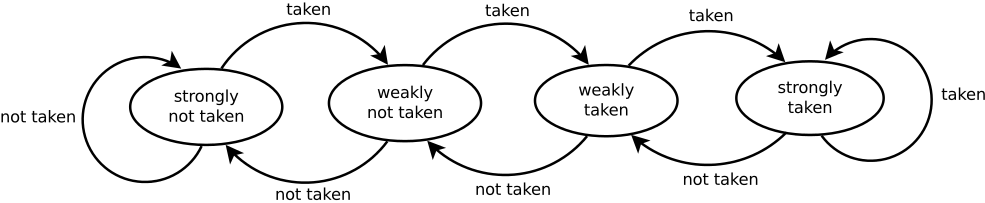
\includegraphics[scale=.35]{bp2bit}
					\caption{Automa di predizione di un one-level branch predictor a 2 bit}
					\label{fig:bp2bits}
				\end{center}
			\end{figure}
		
			Come da schema in \cref{fig:bp2bits} un one-level branch predictor può essere descritto con un semplice automa a 4 stati.
			
			\begin{enumerate}
				\item \emph{Strongly not taken:} in questo stato il \ac{BP} sceglierà il ramo else del branch. In caso di risultato effettivamente negativo resterà in questo stato altrimenti passerà allo stato 2.
				\item \emph{Weakly not taken:} in questo stato il \ac{BP} ha già osservato una esecuzione then ma la sua scelta resterà ancora il ramo else. Se il controllo si rivelerà false, il \ac{BP} tornerà allo stato 1 ma se si rivelerà true andrà allo stato 3 dal quale inizierà a scegliere il ramo then.
				\item \emph{Weakly taken:} come detto in precedenza, in questo stato il \ac{BP} inizierà ad eseguire speculativamente il ramo then. Se da questo stato si ottiene un false, torneremo allo stato 2, altrimenti passeremo al 4.
				\item \emph{Strongly taken:} questo stato è il duale dello stato 1. In questa situazione il \ac{BP} eseguirà il ramo then rimanendo in questo stato se otterrà un true e tornando allo stato 3 se otterrà un false (continuando comunque ad eseguire il ramo then).
			\end{enumerate}
		
			In questo caso vediamo come l'esecuzione consecutiva di al più due rami then ci porta sicuramente in uno stato in cui il ramo scelto dal \ac{BP} sarà sicuramente quello then. Questa informazione sarà molto utile quando dovremo effettuare un training sul \ac{BP} per convincerlo a prendere una certa decisione quando si troverà davanti ad un certo branch.
			
	\section{L'attacco}
		L'attacco SPECTRE induce la vittima ad eseguire speculativamente operazioni che non dovrebbero essere eseguite durante l'esecuzione corretta del programma. Da tali operazioni si otterranno poi le informazioni ricercate tramite un side-channel temporale.
		
		L'attacco si può scomporre in tre fasi:
		
		\begin{enumerate}
			\item \emph{Fase di setup:} in questa fase l'attaccante esegue delle operazioni che convincono il \ac{BP} ad eseguire il ramo then in caso si rendesse necessaria una esecuzione speculativa. In questa fase si cerca anche di costruire tale necessità ad esempio eseguendo letture di memoria che rimuovono dalla cache un valore che sarà poi necessario successivamente. Come ultima cosa l'attaccante può iniziare a preparare la porzione di cache dalla quale estrarrà il valore che vuole carpire alla vittima (ad esempio eseguendo il flush o l'evict di una line o di un set).
			\item \emph{Esecuzione speculativa:} in questa fase il processore esegue speculativamente delle istruzioni che esporrano informazioni confidenziali della vittima recuperabili tramite un side-channel. Tale esecuzione può esporre dati sensibili attraverso una vasta gamma di side-channels ma nell'articolo gli autori si concentrano sulla possibilità di recuperare un valore che risiede ad un indirizzo preciso nella memoria della vittima attraverso un attacco di tipo Flush+Reload o Evict+Reload.
			\item \emph{Recupero del dato:} come ultimo passo, viene montato l'attacco alla cache (Flush+Reload o Evict+Reload). Il recupero del dato si ottiene andando a misurare il tempo necessario alla lettura dall'indirizzo di memoria presente nella line sotto attacco.
		\end{enumerate}
	
		Vediamo adesso un esempio pratico di attacco.
		
		\subsection{Esempio}
		
			Consideriamo il caso di una funzione che contiene al suo interno il seguente codice che riceve un intero x da una fonte non fidata:
			
			\begin{lstlisting}[language={C}, frame={none},basicstyle={\footnotesize}]
				if (x < array1_size) {
					y = array2[array1[x] * 256];
				}
			\end{lstlisting}
			
			Il processo che esegue il codice ha accesso ad un array di bytes \emph{array1} di dimensione \emph{array1\_size} ed un secondo array, \emph{array2}, di dimensione pari a 64KB.
			
			La funzione inizia con un controllo su x, necessario per essere sicuri di non permettere la lettura di porzioni di memoria al di fuori di array1. Durante l'esecuzione speculativa di questo codice però, il \ac{BP} può selezionare il ramo then relativo a questo controllo ad esempio nel seguente caso:
			
			\begin{itemize}
				\item il valore di x viene scelto in maniera malevola in maniera tale da far puntare array1[x] ad un byte segreto \emph{k} che risiede da qualche parte nella memoria della vittima.
				\item \emph{array1\_size} e \emph{array2} non sono presenti nella cache ma \emph{k} lo è.
				\item operazioni precedenti hanno restituito un valore di x corretto, addestrando il \ac{BP} a scegliere il ramo then.
			\end{itemize}
		
			Questa situazione può presentarsi in maniera normale o può essere creata dall'attaccante ad esempio leggendo grandi quantità di memoria per riempire la cache di valori completamente scorrelati ed effettuando una chiamata legittima ad una funzione che utilizzi \emph{k}.
			
			A questo punto, quando il programma inizia a girare il processore esegue il confronto tra x e \emph{array1\_size}. La lettura di \emph{array1\_size} si traduce in un cache miss ed il processore richiede il dato dalla memoria principale. Durante l'attesa il \ac{BP} assume che il risultato dell' \emph{if} sarà \emph{true}, eseguirà speculativamente la somma di x all'indirizzo base di \emph{array1} e richiederà il dato presente all'indirizzo appena calcolato. Questa operazione si tradurrà in una cache hit e verrà restituito molto velocemente il valore del byte segreto \emph{k}. L'esecuzione speculativa continua il suo percorso e verrà calcolato l'indirizzo di \emph{array2[k*256]}. La richiesta del dato contenuto a questo indirizzo si tradurrà in una cache miss e verrà richiesta una lettura dalla memoria principale. Durante questa seconda attesa, al processore arriva finalmente il valore di \emph{array1\_size}. Dopo aver eseguito il confronto il processore si accorge che l'esecuzione speculativa era errata ed esegue un rollback allo stato precedente al branch. Il problema sorge in questo momento. La richiesta di lettura rimasta sospesa viene comunque portata a termine e il valore relativo non viene rimosso dalla cache.
			
			Per completare l'attacco l'attaccante non deve fare altro che rilevare questo cambiamento nello stato della cache per recuperare il byte segreto \emph{k}.
			
			Nel caso più semplice, quello cioè in cui l'attaccante ha accesso diretto ad \emph{array2}, egli non dovrà fare altro che provare  a leggere tutte le posizioni di \emph{array2[n*256]} per tutti i valori di $n \in (0\dots255)$. Solamente uno di questi sarà presente in cache (quello per \emph{n} = \emph{k}) e verrà restituito velocemente mentre tutti gli altri verranno restituiti in tempi molto lunghi. Prendendo l'unico valore restituito in tempo breve, l'attaccante avrà trovato il byte segreto \emph{k}.
			
			Questo attacco può ovviamente essere eseguito un numero indeterminato di volte e può portare alla completa lettura della memoria della vittima un byte alla volta.
			
	\section{Le contromisure}
		Come detto all'inizio del capitolo, al momento attuale non sono state rilasciate patch a livello di hardware o di microprogrammazione del processore in grado di risolvere completamente il problema.
		
		La soluzione più ovvia è quella di non permettere l'esecuzione speculativa tout court ma questa scelta andrebbe ad impattare eccessivamente sulle prestazioni. L'idea è quella di cercare di impedire l'esecuzione speculativa su parti di codice compromettenti.
		
		In questa direzione, sia Intel che AMD, nei loro white papers \cite{AMD2018speculation,intel2018speculative}, suggeriscono alcune regole di programmazione per difendersi da questi attacchi.
		
		\subsection{Serializzare gli accessi alla memoria}
		
		La prima regola è quella di serializzare gli accessi alla memoria tramite l'utilizzo dell'istruzione \emph{lfence()}\index{Lfence()}. Questa è un tipo di istruzione di \emph{barriera} che forza il processore o il compilatore ad una esecuzione ordinata delle operazioni di memoria richieste immediatamente prima ed immediatamente dopo la barriera. Tipicamente questo fa sì che sia garantito che l'istruzione che segue la barriera non venga eseguita prima di quella che la precede. A titolo di esempio, analizziamo i seguenti codici:
		
		\begin{lstlisting}[language={C},frame={blrt},basicstyle=\footnotesize,numbers=left,numberstyle=\scriptsize\color{black}]
			if (user_value >= LIMIT) {
				return ERROR;
			} 
			x = table[user_value]; 
			node = entry[x];
		\end{lstlisting}
		
		\begin{lstlisting}[language={C},frame={rlbt},basicstyle=\footnotesize,numbers=left,numberstyle=\scriptsize\color{black}]
		if (user_value >= LIMIT) {
			return ERROR;
		} 
		lfence(); 
		x = table[user_value]; 
		node = entry[x];
		\end{lstlisting}
		
		Nel primo caso, la riga 4 può essere eseguita speculativamente con il valore \emph{user\_value} fornito dall'attaccante mentre si attende il risultato del controllo presente alla riga 1, ritardato perché il valore di \emph{LIMIT} non è presente in cache.
		
		L'istruzione \emph{lfence()} alla riga 4 del secondo codice scongiura questa eventualità impedendo l'accesso alla memoria prima che sia terminato l'accesso precedente. 
		
		Questa soluzione sicuramente risolve il problema ma ha due grossi difetti; deve essere inserita manualmente a livello di programmazione e porta una perdita di prestazioni notevole\cite{AMD2018speculation}.
		
		Microsoft implementa nel proprio compilatore una rilevazione automatica del codice vulnerabile agli attacchi di tipo SPECTRE ed inserisce tali barriere automaticamente. Purtroppo la blacklist di questo strumento comprende solamente le situazioni più comuni e maggiormente utilizzat. Kocher infatti dimostra che tale analisi automatica non rileva molte sezioni di codice vulnerabile\cite{kocher2018mitigation}.
\chapter{SPARK}
	In questo capitolo verrà analizzato \ac{SPARK}\index{SPARK}, il nostro attacco basato sul progetto SPECTRE capace di recuperare chiavi (o più in generale "segreti") evitando il controllo della password.
	
	\section{Scenario}
		Immaginiamo di partire dalla funzione attaccata da SPECTRE (\cref{list:vulnerabile}). Nello scenario più semplice si può pensare che \emph{array1} (da adesso sarà chiamato \emph{secret}) contenga delle chiavi predefinite assegnate ad ogni utente che vengono utilizzate come indici  per accedere ad \emph{array2} che contiene le informazioni riservate di tutti gli utenti. Dato che queste informazioni sono riservate, il tutto è protetto con una password. 
		
		L'utente \emph{x}, identificato tramite il proprio \emph{userID}, che vuole consultare i propri dati dovrà inserire ID e password (salvate nell'array delle password \emph{passwordDigest}). In caso di controllo positivo, si utilizzerà l'indice contenuto in \arr{secret}{userID} per andare a recuperare l'informazione che si riferisce ad \emph{x}. In caso di controllo negativo verrà ovviamente negato l'accesso ai dati.
		
		Tale funzione potrebbe essere implementata dal \cref{list:spark}:
		\codice{28}{32}{Funzione attaccata da SPARK}{list:spark}
		
		Supponiamo adesso che l'attaccante abbia accesso ad \emph{array2} (come supposto anche dall'attacco SPECTRE) ma che non abbia accesso a \emph{secret} ed ovviamente neanche all'array delle password. L'obiettivo del nostro attacco è quello di ricavare, per un utente casuale \emph{x}, il rispettivo \arr{secret}{x}, per poter successivamente avere accesso all'informazione riservata, il tutto senza conoscere la password.
		
		La precisione del risultato ottenuto dipende molto dal processore e dal tipo di dati utilizzato per rappresentare i vari valori. Nella nostra implementazione abbiamo utilizzato il tipo di dato \emph{int} grande trentadue bit; questo, in una cache con dimensione delle line pari a 512 bit (un valore considerato standard nei processori più moderni) non ci permette di recuperare esattamente \arr{secret}{x} (\cref{fig:lineSize}) ma di localizzarlo entro un certo intervallo \arr{secret}{x} $\pm \ \delta$ con, $$\delta = \frac{\text{dimensione di una line}}{\text{dimensione del tipo di dato}} = \frac{512}{32} = 16.$$
		
		\begin{figure}
			\begin{center}
				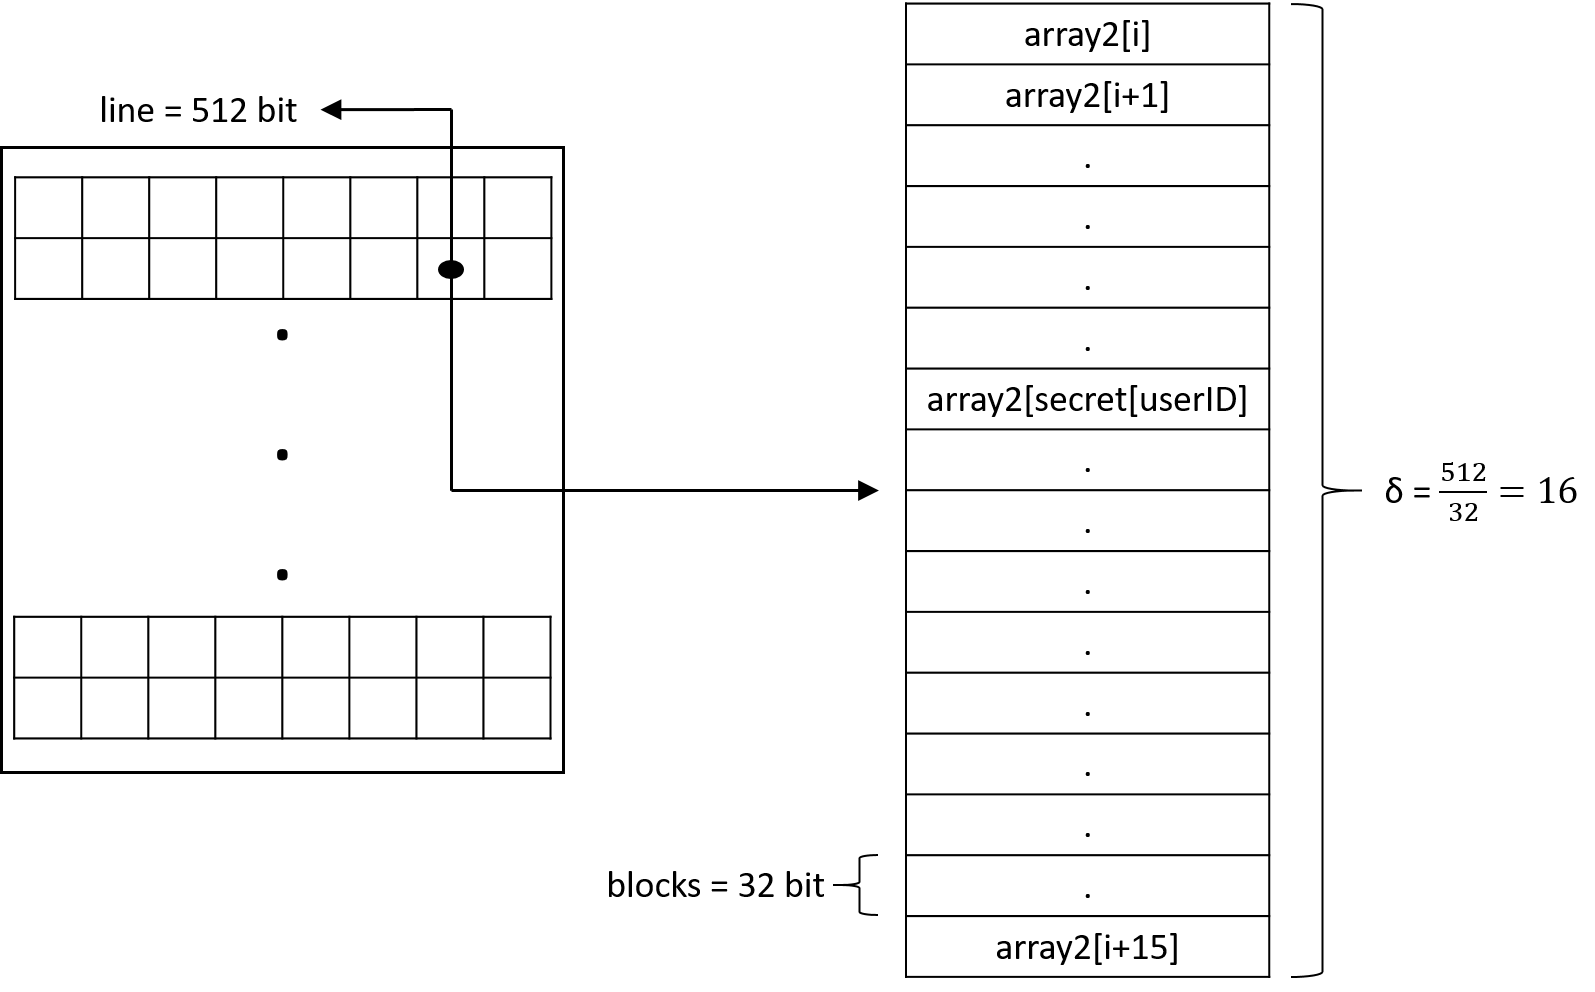
\includegraphics[width=.8\textwidth]{lineSize}
				\caption{Contenuto di una cache line nel nostro setup}
				\label{fig:lineSize}
			\end{center}
		\end{figure}
		
		\section{L'attacco}
			Prima di analizzare l'effettiva implementazione, vediamo l'idea generale dell'attacco che può essere suddiviso in quattro parti:
			
			\begin{enumerate}
				\item Il \ac{BP} viene addestrato richiamando la funzione vittima per tre volte con uno \emph{userID} e la relativa password corretta. Questo risultato è facilmente ottenibile dall'attaccante utilizzando i propri dati di accesso.
				\item Viene eseguito il \emph{flush} dalla cache di tutti i dati relativi ad \emph{array2} e \emph{passwordDigest}. Ricordiamo che l'istruzione \emph{clflush} non richiede alcun privilegio per essere eseguita.
				\item Viene richiamata la funzione vittima con lo \emph{userID} di cui vogliamo scoprire il segreto (chiamato \emph{userUnderAttack}) ed una password casuale.
				\item Si calcola il tempo necessario all'accesso di tutte le posizioni di \emph{array2}. Considerato che l'unico dato relativo ad \emph{array2} presente in cache in questo momento è \emph{y} = \arrdoppio{array2}{secret}{userUnderAttack} (per la chiamata precedente), solamente per questo otterremo un tempo basso mentre per tutti gli altri sarà alto perché dovranno essere recuperati dalla memoria principale.
			\end{enumerate}
		
			L'attacco funziona sfruttando l'esecuzione speculativa del processore sul controllo della password. Avendo eseguito il \emph{flush} di \emph{passwordDigest} al punto 2, \arr{passwordDigest}{userUnderAttack} non sarà presente in cache al momento del controllo al punto 3. Nell'attesa del suo recupero dalla memoria principale, il \ac{BP} eseguirà il ramo \emph{then} della computazione a causa dell'addestramento ottenuto al punto 1. Verrà richiesto dalla memoria \emph{y} che verrà caricato in cache. Quando sarà disponibile \arr{passwordDigest}{userUnderAttack}, il controllo fallirà e non verrà permesso l'accesso ai dati ma \emph{y} resterà in cache. A questo punto, accedendo a tutte le posizioni \arr{array2}{l} con \emph{l} $\in (0,\dots,\text{\emph{size(array2)}}-1)$ , l'unica che ci darà una risposta veloce sarà \emph{l} = \arr{secret}{userUnderAttack} e avremo così scoperto il valore segreto.
			
			\subsection{Implementazione}
				Passiamo adesso all'analisi dettagliata del codice C che implementa l'attacco.
				
				\subsubsection{Inizializzazione}
				\codspark{1}{22}
				
				Nella primissima parte del nostro programma vengono semplicemente caricate le librerie necessarie alla compilazione, viene definito il numero di utenti (tremila), vengono creati i tre array principali \emph{secret},\emph{array2} e \emph{passwordDigest} e viene definita la funzione vittima, esattamente la stessa proposta nello scenario.
				
 				La libreria \emph{x86intrin} fornisce le istruzioni \emph{rdtscp} e \emph{\_\_mm\_clflush} necessarie al calcolo dei tempi di hit e al flush della cache. In particolare l'istruzione \emph{\_\_mm\_clflush} prende come argomento un indirizzo di memoria ed invalida, su tutti i livelli della cache, tutte le line che contengono quell'indirizzo.
				
				I tre array "utili" sono separati da altri array \emph{unused} per essere sicuri che vengano distanziati in memoria. Questo fa sì che non si sovrappongano all'interno di una stessa line.
				
				\subsubsection{Main - definizione parametri}
				\codspark{24}{52}
				
				In questa parte vengono definiti i parametri che verranno utilizzati nel resto del programma:

					\emph{CACHELINE}: La dimensione in bit di una singola cache line. Come già detto, questa dimensione è ormai standardizzata a 512 bit su tutti i processori moderni.
					
					\emph{blocks}: La dimensione in bit di un singolo elemento dell'array. In questo caso 32 bit.
					
					\emph{delta}: Il numero di elementi dell'array che sono contenuti in una cache line.
					
					\emph{class}: Il numero di classi di risultati \emph{mod} $\delta$ ottenute.
					
					\emph{numberOfRuns}: Il numero di volte che viene eseguito l'attacco per ogni esperimento.
					
					\emph{numberOfTests}: Il numero di esperimenti che vengono eseguiti.
					
					\emph{cacheHitThreshold}: Il valore di soglia entro il quale si considera una cache hit. Sperimentalmente questo valore si aggira tra i 30 e i 40 cicli di clock.
					
					\emph{precisionLoss}: Con questo valore si regola la precisione che si vuole ottenere. Se lasciato a zero verrà restituito l'intervallo ($x-\delta, x+\delta$) che dovrebbe contenere il segreto. A volte però può succedere che venga fornito un intervallo che non contiene il segreto a causa di interferenze con altri processi che utilizzano il processore. Aumentando questo valore si aumenta l'intervallo proporzionalmente a $\delta$ perdendo un po' in precisione ma guadagnando in correttezza dell'intervallo.
					
					Questo e i tre precedenti sono i quattro parametri richiesti all'avvio del programma.
					
					\emph{results}: L'array nel quale verranno salvati i risultati.
					
					\emph{ok, error e no-hit}: Tre contatori utilizzati per sapere quante volte il programma trova il segreto, quante volte lo sbaglia e quante volte non rileva nessun cache hit.
					
					\emph{timeReg, time1 e time2}: Le tre variabili per calcolare i tempi di accesso alle posizioni di \emph{array2}.
			
				Dopo aver definito tutti i parametri si procede con l'inizializzazione del generatore \emph{srand} di numeri casuali.
				
				\subsubsection{Main - inizializzazione dell'esperimento}
				\codspark{54}{70}
				
				All'inizio di ogni test viene scelto casualmente lo \emph{userUnderAttack} e vengono inizializzati casualmente i tre array principali \emph{passwordDigest, array2} e \emph{secret}. Successivamente si sceglie una password sicuramente sbagliata ed infine si prepara l'array \emph{result} alla ricezione dei risultati settandolo a zero.
				
				\subsubsection{Main - l'attacco}
				\codspark{72}{99}
				
				Come descritto nello scenario, l'attacco si divide in quattro parti. Nella prima parte viene addestrato il \ac{BP} ad eseguire speculativamente il ramo then della funzione vittima richiamandola per tre volte con \emph{userID} e password corretta.
				
				Successivamente si esegue il flush dalla cache di tutte le posizioni degli array \emph{array2} e \emph{passwordDigest}.
				
				Prima di richiamare la funzione vittima abbiamo messo l'istruzione \emph{\_mm\_lfence}. Tale istruzione è una barriera sulla memoria che non permette l'esecuzione delle istruzioni successive prima che siano terminate tutte le scritture in memoria delle istruzioni precedenti. Questo evita ad esempio che l'istruzione a riga 90 venga eseguita prima del flush di \emph{array2} a causa di un riordinamento del codice. Se accadesse questo, il risultato del calcolo del tempo di accesso sarebbe ovviamente falsato.
				
				Terminato il flush della cache, viene richiamata la funzione vittima e vengono calcolati i tempi di accesso alle varie posizioni di \emph{array2}. Come si può notare, non si effettua l'accesso a tutte le posizioni di \emph{array2} ma si procede con un passo $\delta$ visto che comunque una qualunque delle $\delta$ posizioni all'interno della line restituirà una hit.
				
				Con un'altra \emph{\_mm\_lfence} ci assicuriamo che il tempo venga effettivamente salvato in \emph{time2} ed effettuiamo il controllo. Se il risultato del calcolo del tempo di accesso è minore della soglia che abbiamo impostato, aumentiamo di uno nell'array \emph{results} il valore  contenuto all'indice che stiamo analizzando.
\appendix
\chapter{SPARK - Codice completo}

	\lstinputlisting[language={C},frame={none},basicstyle={\scriptsize},caption={SPARK - codice completo} ]{"D:/UNIFI/Magistrale/Tesi/spectre/primeProbe/spark.c"}
%-----------------BIBLIOGRAFIA---------------------------------
\bibliography{bib/bibliografia}
\bibliographystyle{unsrt}
%--------------------------------------------------------------
\addcontentsline{toc}{chapter}{Acronimi}
\chapter*{Acronimi}
\begin{acronym}[CAGD]
	\acro{AES}{Advanced Encryption Standard}
	\acro{CNES}{Centre National d’Etudes Spatiales}
	\acro{DES}{Data Encryption Standard}
	\acro{DPA}{Differential Power Analysis}
	\acro{HTTPS}{HyperText Transfer Protocol over Secure Socket Layer}
	\acro{LED}{Light Emitting Diode}
	\acro{PICA}{Picosecond Imaging Circuit Analysis}
	\acro{SPA}{Simple Power Analysis}
  	\acro{USB}{Universal Serial Bus}
\end{acronym}
\printindex
\end{document}
%--------------------------------------------------------------
